%%%%%%%%%%%%%%%%%%%%%%%%%%%%%%%%%%%%%%%%%%%%%%%%%%%%%%%%%%%%%%%%%%%%%%%%%%%%%%%

\section{$\Pi$ berechnen}

Wir stellen uns die Frage, in welchem Verhältnis die Fläche eines Qudrates zu der Fläche des in dieses Quadrat eingeschriebenen Kreises ist. 

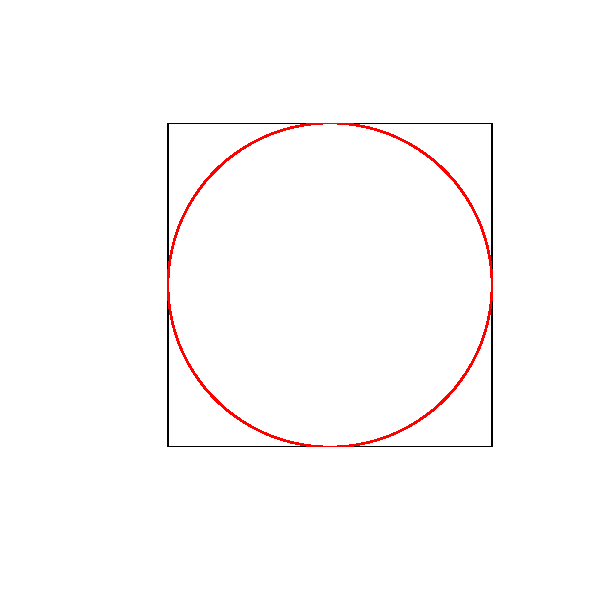
\includegraphics{sim_pi-001}

Die Kantenlänge des Quadrates sei $2r=2$ somit hat der Kreis den Radius $r=1$. Die Fläche des Kreises ist folglich $\pi r^2 = \pi 1^2 = \pi$. Die Fläche des Quadrats ist $(2r)^2=4$. Das Verhältnis der beiden Flächen zueinander ist somit:

\begin{equation} \label{eq:pi}
  \rho = \frac{\text{Fläche des Kreises}}{\text{Fläche des Quadrats}} = \frac{\pi r^2}{(2r)^2} = \frac{\pi}{4}
\end{equation}

Die Herangehensweise ist nun zufällig Punkte innerhlab des Quadrates zu erzeugen. Im nächten Schritt werden die Punkte, die innerhalb und außerhalb des Kreises fallen ausgezählt Das Verhätnis zwischen ihnen multipliziert mit 4 ist eine Schätzung von $\pi$.
Um die Punkte innerhlab des Kreieses zu bestimmen berechnen wir ihren Abstand vom Zentrum. Dieser darf maximal $1$ betragen.

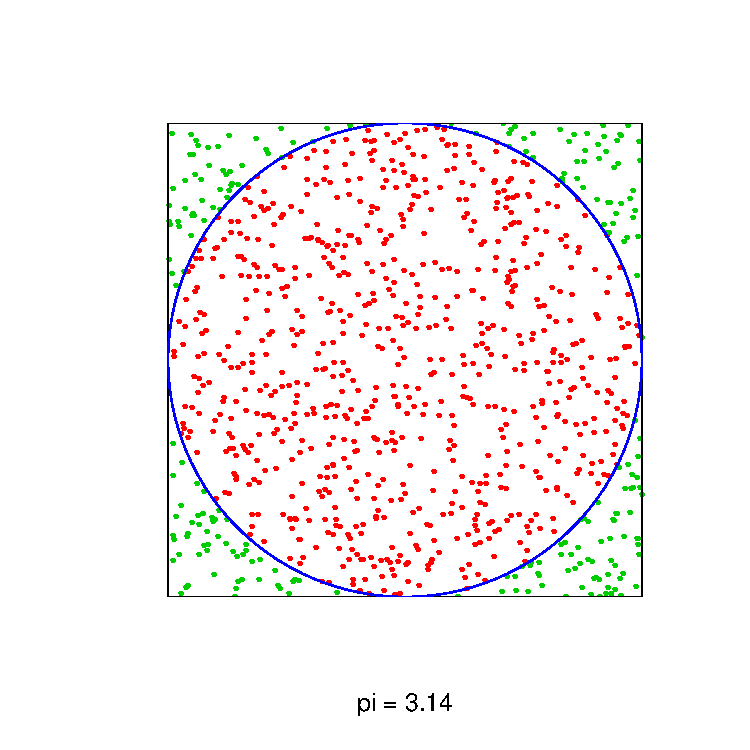
\includegraphics{sim_pi-002}

Berechnen wir nun dieses Verhältnis für eine größere Anzahl an Punkten. Um den Abstand von Zentrum zu berechnen wird die euklidische Distanz genutzt, $\sqrt{x^2 + y^2}$. Alle Punkte mit einer Distanz kleiner gleich Eins liegen innerhalb des Kreises.
          
\begin{Schunk}
\begin{Sinput}
> estimate_pi <- function(n=10e4){
+   x <- runif(n, -1, 1)                # Zufällige x Werte 
+   y <- runif(n, -1, 1)                # Zufällige y Werte
+   z <- sqrt(x^2 + y^2)                # Abstand zum Ursprung
+   n.in.circle <- length(z[z <= 1])    # Anzahl an Punkten im Kreis
+   n.in.circle / n * 4                 # Verhältnis * 4
+ } 
> estimate_pi(10e4)
\end{Sinput}
\begin{Soutput}
[1] 3.13904
\end{Soutput}
\end{Schunk}

Die Schätzung funktioniert. Der letzte Schritt in eier Simulation ist es häufig den Code schneller zu machen. In unseren Fall ist dies nciht wichtig, da die Simulation nur wenige Sekunden dauert. Bei längeren Simulationen könne so jedoch Stunden oder gar Tage an Rechenzeit eingespart werden. Unser Ziel ist es hier, alle Operationen, die nicht nötig sind wegzulassen. Um die Laufzeit der Simulation zu überpfüfen kann die Funktion \texttt{system.time} genutzt werden.

\begin{Schunk}
\begin{Sinput}
> system.time({
+   estimate_pi(10e5)
+ })   
\end{Sinput}
\begin{Soutput}
   user  system elapsed 
  0.161   0.056   0.256 
\end{Soutput}
\end{Schunk}

Nehmen wir nun eineige Verbessrungen vor. Da wir nur wissen wollen, welche Werte kleiner oder gleich Eins sind ist die Wurzeloperation nicht nötig. Darüber hinaus kann auch beim Auszählen der Punkte im Kreis eine Operation gespart werden.

\begin{Schunk}
\begin{Sinput}
> estimate_pi_2 <- function(n=10e4){
+   x <- runif(n, -1, 1)
+   y <- runif(n, -1, 1) 
+   z <- x^2 + y^2                    # keine Wurzel
+   n.in.circle <- sum(z <= 1)        # kein Vektorzugriff 
+   n.in.circle / n * 4  
+ } 
\end{Sinput}
\end{Schunk}

\begin{Schunk}
\begin{Sinput}
> system.time({
+   estimate_pi_2(10e5)
+ })   
\end{Sinput}
\begin{Soutput}
   user  system elapsed 
  0.132   0.037   0.235 
\end{Soutput}
\end{Schunk}

Die Performance hat sich durch diese Schritte um gut $25\,\%$ verbessert. Eliminieren wir zuletzt noch einige unnötige Speicherschritte.

\begin{Schunk}
\begin{Sinput}
> estimate_pi_3 <- function(n=10e4){ 
+   z <- runif(n, -1, 1)^2 + 
+        runif(n, -1, 1)^2
+   sum(z <= 1) / n * 4 
+ } 
\end{Sinput}
\end{Schunk}

\begin{Schunk}
\begin{Sinput}
> system.time({
+   estimate_pi_3(10e6)
+ })   
\end{Sinput}
\begin{Soutput}
   user  system elapsed 
  1.469   0.446   2.497 
\end{Soutput}
\end{Schunk}

Die Performance hat sich so erneut um ca. $20\,\%$ verbessert. 

%%%%%%%%%%%%%%%%%%%%%%%%%%%%%%%%%%%%%%%%%%%%%%%%%%%%%%%%%%%%%%%%%%%%%%%%%%%%%%%
